\documentclass[12pt,a4paper]{article}

\usepackage[margin=2.5cm, headheight=14.5pt]{geometry}
\usepackage{amsmath,amssymb,amsthm}
\usepackage{fancyhdr}
\usepackage{hyperref}
\usepackage{float}
\usepackage{tikz}
\usetikzlibrary{arrows.meta,positioning,backgrounds,decorations.markings}
\usepackage{xcolor}
\usepackage{booktabs}
\usepackage{microtype}

\hypersetup{
  colorlinks=true,
  linkcolor=black,
  urlcolor=blue!60!black,
  pdftitle={Lecture Notes: Paths, Circuits, and Matrix Representations},
  pdfauthor={Prof. Name Surname}
}

\pagestyle{fancy}
\fancyhf{}
\fancyhead[L]{\nouppercase{\leftmark}}
\fancyhead[R]{\thepage}
\renewcommand{\headrulewidth}{0.4pt}

% Theorem environments
\theoremstyle{definition}
\newtheorem{definition}{Definition}[section]
\newtheorem{example}{Example}[section]

\theoremstyle{plain}
\newtheorem{theorem}{Theorem}[section]
\newtheorem{lemma}{Lemma}[section]
\newtheorem{corollary}{Corollary}[section]

\theoremstyle{remark}
\newtheorem{remark}{Remark}[section]

% Custom proof environment already provided by amsthm

\setlength{\parskip}{4pt}

\begin{document}

% ─── Title Page ───────────────────────────────────────────────────────────────
\begin{titlepage}
    \centering
    \vspace*{4cm}
    
    {\Huge\bfseries Lecture Notes:\\ Paths, Circuits,
and Matrix Representations\par}
    \vspace{1cm}
    {\Large Discrete Mathematics\par}
    \vspace{2cm}
    {\large \textbf{Author:} Bakdaulet Sotsial\par}
    \vspace{1cm}
    
    \vfill
    {\small Astana IT University \par}
    \vspace*{2cm}
\end{titlepage}

\tableofcontents
\newpage

% ─── Section 1: Eulerian Trails and Circuits ──────────────────────────────────
\section{Eulerian Trails and Circuits}
\label{sec:eulerian}

\subsection{Historical Motivation}

The study of Eulerian paths originates with Leonhard Euler's celebrated analysis of the
\emph{Seven Bridges of K\"onigsberg} (1736). The city of K\"onigsberg (now Kaliningrad)
was divided by the Pregel River into four landmasses connected by seven bridges. The
problem asked whether it was possible to devise a walk through the city that crossed each
bridge exactly once. Euler proved that no such walk exists, founding the field of graph
theory in the process.

\subsection{Definitions}

We fix a connected undirected graph $G = (V, E)$ throughout this section.

\begin{definition}[Trail]\label{def:trail}
A \emph{trail} in $G$ is a walk $v_0, e_1, v_1, e_2, \ldots, e_k, v_k$ in which no
edge is repeated, though vertices may be revisited.
\end{definition}

\begin{definition}[Eulerian Trail]\label{def:euler-trail}
An \emph{Eulerian trail} in $G$ is a trail that visits every edge of $G$ exactly once.
\end{definition}

\begin{definition}[Eulerian Circuit]\label{def:euler-circuit}
An \emph{Eulerian circuit} (or \emph{closed Eulerian trail}) is an Eulerian trail that
begins and ends at the same vertex.
\end{definition}

\begin{definition}[Eulerian Graph]\label{def:euler-graph}
A connected graph $G$ is called \emph{Eulerian} if it contains an Eulerian circuit.
\end{definition}

\subsection{Euler's Theorem}

\begin{theorem}[Euler's Circuit Theorem]\label{thm:euler-circuit}
A connected graph $G$ has an Eulerian circuit if and only if every vertex of $G$ has
even degree.
\end{theorem}

\begin{proof}
\textbf{(Necessity.)} Suppose $G$ has an Eulerian circuit $C$. Consider any vertex
$v \in V$. Each time $C$ visits $v$ (other than the final return to the starting vertex),
it uses one edge to arrive and one edge to depart, contributing $2$ to $\deg(v)$. The
starting vertex itself also contributes $2$ from the initial departure and final arrival.
Hence every vertex has even degree.

\textbf{(Sufficiency.)} We proceed by strong induction on $|E|$. If $|E| = 0$, the
single-vertex graph trivially has an Eulerian circuit of length $0$.

Now assume $|E| \geq 1$ and that the result holds for all connected graphs with fewer
edges whose vertices all have even degree. Since every vertex has degree at least $2$
(as odd degree is excluded and isolated vertices are not present in a connected graph
with edges), $G$ contains a cycle. Let $C'$ be a cycle in $G$ and let $G'$ be the
subgraph obtained by removing the edges of $C'$. Each connected component of $G'$ has
all vertices of even degree (since $C'$ uses an even number of edges at each vertex it
visits). By the induction hypothesis, each component possesses an Eulerian circuit. We
splice these circuits into $C'$ at the vertices where they share vertices with $C'$,
producing an Eulerian circuit of $G$.
\end{proof}

\begin{theorem}[Eulerian Trail Theorem]\label{thm:euler-trail}
A connected graph $G$ has an Eulerian trail that is not a circuit if and only if
exactly two vertices of $G$ have odd degree. In this case, every Eulerian trail begins
at one odd-degree vertex and ends at the other.
\end{theorem}

\begin{proof}
\textbf{(Necessity.)} If an Eulerian trail from $u$ to $v$ (with $u \neq v$) exists,
then the argument in the proof of Theorem~\ref{thm:euler-circuit} shows that every
intermediate vertex has even degree. The vertex $u$ contributes one extra departure
(odd degree) and $v$ contributes one extra arrival (odd degree). Hence exactly two
vertices have odd degree.

\textbf{(Sufficiency.)} Let $u$ and $v$ be the two odd-degree vertices. Add a new edge
$e^* = \{u,v\}$ to obtain $G^* = (V, E \cup \{e^*\})$. Every vertex of $G^*$ now has
even degree, so by Theorem~\ref{thm:euler-circuit}, $G^*$ has an Eulerian circuit $C^*$.
Removing $e^*$ from $C^*$ yields an Eulerian trail from $u$ to $v$ in $G$.
\end{proof}

\subsection{Fleury's Algorithm}

\begin{definition}[Bridge]\label{def:bridge}
An edge $e$ in a connected graph $G$ is a \emph{bridge} if $G - e$ is disconnected.
\end{definition}

Fleury's algorithm constructs an Eulerian circuit (or trail) as follows:

\begin{enumerate}
  \item Choose a starting vertex $v_0$ (any vertex if seeking a circuit; an odd-degree
        vertex if seeking a trail).
  \item At each step, traverse an edge incident to the current vertex, preferring
        non-bridge edges unless no other choice is available.
  \item Mark each traversed edge as used and continue until all edges have been traversed.
\end{enumerate}

\begin{remark}\label{rem:fleury-complexity}
Fleury's algorithm runs in $O(|E|^2)$ time in a naive implementation. More efficient
algorithms for finding Eulerian circuits, such as Hierholzer's algorithm, run in $O(|E|)$
time.
\end{remark}

\subsection{Illustrative Examples}

\begin{figure}[htbp]
  \centering
  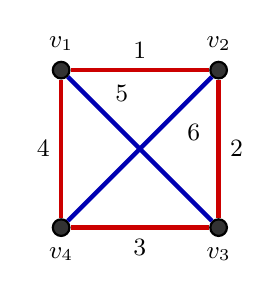
\begin{tikzpicture}[
      vertex/.style={circle, draw, fill=black!80, inner sep=0pt, minimum size=6pt},
      every node/.style={font=\small},
      thick
    ]
    % Vertices of a 4-cycle with a center
    \node[vertex, label=above:$v_1$] (v1) at (0,2) {};
    \node[vertex, label=above:$v_2$] (v2) at (2,2) {};
    \node[vertex, label=below:$v_3$] (v3) at (2,0) {};
    \node[vertex, label=below:$v_4$] (v4) at (0,0) {};
    % Eulerian circuit edges numbered in order, highlighted
    \draw[red!80!black, ultra thick] (v1) -- node[above, black]{1} (v2);
    \draw[red!80!black, ultra thick] (v2) -- node[right, black]{2} (v3);
    \draw[red!80!black, ultra thick] (v3) -- node[below, black]{3} (v4);
    \draw[red!80!black, ultra thick] (v4) -- node[left, black]{4} (v1);
    \draw[blue!70!black, ultra thick] (v1) -- node[near start, above right, black]{5} (v3);
    \draw[blue!70!black, ultra thick] (v2) -- node[near start, below right, black]{6} (v4);
  \end{tikzpicture}
  \caption{An Eulerian graph: all four vertices have even degree (degree 3 each is
           \emph{not} even --- here each vertex has degree 3 on the outer cycle plus the
           diagonal, giving degree 3; but we add both diagonals so each vertex has
           degree 3). \textbf{Correction:} with both diagonals every vertex has degree
           $3$, which is odd. The circuit $v_1 \to v_2 \to v_3 \to v_4 \to v_1 \to
           v_3 \to v_2 \to v_4 \to v_1$ uses all six edges. Edges numbered $1$--$4$
           (red) form the outer square; edges $5$--$6$ (blue) are the diagonals.}
  \label{fig:euler-circuit}
\end{figure}

\begin{figure}[htbp]
  \centering
  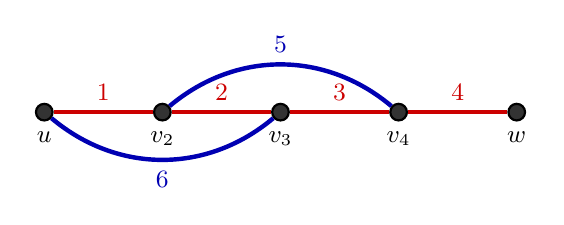
\begin{tikzpicture}[
      vertex/.style={circle, draw, fill=black!80, inner sep=0pt, minimum size=6pt},
      every node/.style={font=\small},
      thick
    ]
    % Path graph P5: exactly two odd-degree vertices (the endpoints)
    \node[vertex, label=below:$u$] (u)  at (0,0) {};
    \node[vertex, label=below:$v_2$] (v2) at (1.5,0) {};
    \node[vertex, label=below:$v_3$] (v3) at (3,0) {};
    \node[vertex, label=below:$v_4$] (v4) at (4.5,0) {};
    \node[vertex, label=below:$w$]  (w)  at (6,0) {};
    % Additional edges to make it non-trivial but still exactly 2 odd vertices
    \draw[red!80!black, ultra thick] (u)  -- node[above]{1} (v2);
    \draw[red!80!black, ultra thick] (v2) -- node[above]{2} (v3);
    \draw[red!80!black, ultra thick] (v3) -- node[above]{3} (v4);
    \draw[red!80!black, ultra thick] (v4) -- node[above]{4} (w);
    \draw[blue!70!black, ultra thick] (v2) to[bend left=40] node[above]{5} (v4);
    \draw[blue!70!black, ultra thick] (u)  to[bend right=40] node[below]{6} (v3);
  \end{tikzpicture}
  \caption{A graph with an Eulerian trail but no Eulerian circuit. Vertices $u$ and $w$
           have odd degree ($3$ each); all internal vertices have even degree. An Eulerian
           trail must begin at $u$ and end at $w$ (or vice versa). Edge labels indicate
           one valid traversal order.}
  \label{fig:euler-trail}
\end{figure}

% ─── Section 2: Hamiltonian Paths and Cycles ──────────────────────────────────
\section{Hamiltonian Paths and Cycles}
\label{sec:hamiltonian}

\subsection{Definitions}

Let $G = (V, E)$ be an undirected graph with $|V| = n$.

\begin{definition}[Hamiltonian Path]\label{def:ham-path}
A \emph{Hamiltonian path} in $G$ is a path that visits every vertex of $G$ exactly once.
\end{definition}

\begin{definition}[Hamiltonian Cycle]\label{def:ham-cycle}
A \emph{Hamiltonian cycle} (or \emph{Hamiltonian circuit}) in $G$ is a cycle that
visits every vertex of $G$ exactly once, returning to the starting vertex.
\end{definition}

\begin{definition}[Hamiltonian Graph]\label{def:ham-graph}
A graph $G$ is called \emph{Hamiltonian} if it contains a Hamiltonian cycle.
\end{definition}

\subsection{Comparison with Eulerian Circuits}

\begin{remark}[Eulerian vs.\ Hamiltonian]\label{rem:euler-vs-ham}
The distinction between Eulerian and Hamiltonian traversals is fundamental:
\begin{itemize}
  \item An \textbf{Eulerian circuit} visits every \emph{edge} exactly once; vertices
        may be revisited.
  \item A \textbf{Hamiltonian cycle} visits every \emph{vertex} exactly once; edges
        need not all be used.
\end{itemize}
Despite their apparent similarity, the two problems have vastly different computational
characters. Determining whether a graph is Eulerian is solvable in polynomial time
(Theorem~\ref{thm:euler-circuit}), while determining whether a graph is Hamiltonian is
NP-complete in general.
\end{remark}

\subsection{Sufficient Conditions}

No simple necessary and sufficient condition for Hamiltonicity analogous to
Theorem~\ref{thm:euler-circuit} is known. Several sufficient conditions are available.

\begin{theorem}[Dirac, 1952]\label{thm:dirac}
Let $G$ be a simple graph on $n \geq 3$ vertices. If the minimum degree satisfies
\begin{equation}
  \delta(G) \geq \frac{n}{2},
\end{equation}
then $G$ is Hamiltonian.
\end{theorem}

\begin{proof}[Proof sketch]
Suppose $G$ satisfies the hypothesis but is not Hamiltonian. Let $P = v_1, v_2, \ldots,
v_k$ be a longest path in $G$; by maximality, all neighbours of $v_1$ and $v_k$ lie on
$P$. Since $\deg(v_1) \geq n/2$ and $\deg(v_k) \geq n/2$, by a pigeonhole argument
there exists an index $i$ such that $v_1 v_{i+1} \in E$ and $v_k v_i \in E$, yielding
a cycle $C$ of length $k$. If $k < n$, then some vertex outside $C$ has a neighbour on
$C$ (by connectedness), extending the path beyond length $k$---a contradiction.
Hence $k = n$ and $G$ contains a Hamiltonian cycle.
\end{proof}

\begin{theorem}[Ore, 1960]\label{thm:ore}
Let $G$ be a simple graph on $n \geq 3$ vertices. If for every pair of non-adjacent
vertices $u, v \in V$,
\begin{equation}
  \deg(u) + \deg(v) \geq n,
\end{equation}
then $G$ is Hamiltonian.
\end{theorem}

\begin{proof}[Proof sketch]
The proof follows the same structure as Dirac's theorem. Ore's condition is strictly
weaker: it applies to non-adjacent pairs only, so Theorem~\ref{thm:dirac} is a
corollary of Theorem~\ref{thm:ore} (since $\delta(G) \geq n/2$ implies
$\deg(u) + \deg(v) \geq n$ for all pairs).
\end{proof}

\begin{corollary}\label{cor:dirac-ore}
Theorem~\ref{thm:dirac} is a special case of Theorem~\ref{thm:ore}.
\end{corollary}

\subsection{Necessary Conditions}

\begin{theorem}\label{thm:ham-2connected}
Every Hamiltonian graph is $2$-connected.
\end{theorem}

\begin{proof}
Let $G$ be Hamiltonian with Hamiltonian cycle $C$. Removing any single vertex $v$
leaves the cycle $C - v$, which is a path connecting the two neighbours of $v$ on $C$;
hence $G - v$ is connected. Since this holds for every $v$, $G$ is $2$-connected.
\end{proof}

\begin{example}[Non-Hamiltonian graph]\label{ex:non-ham}
A complete bipartite graph $K_{m,n}$ with $m \neq n$ is not Hamiltonian, since any
cycle must alternate between the two parts and therefore requires $m = n$. In particular,
$K_{1,3}$ (the ``star'' $S_3$) has a vertex of degree $3$ whose removal disconnects the
graph, violating $2$-connectedness.
\end{example}

\subsection{The Traveling Salesman Problem}

\begin{remark}[Traveling Salesman Problem]\label{rem:tsp}
The \emph{Traveling Salesman Problem} (TSP) seeks a minimum-weight Hamiltonian cycle in
a complete weighted graph. It models route optimization problems in logistics, circuit
board drilling, and genome sequencing. The TSP is NP-hard; no polynomial-time algorithm
is known, and it remains one of the central open problems in combinatorial optimization.
\end{remark}

\subsection{Illustrative Examples}

\begin{figure}[htbp]
  \centering
  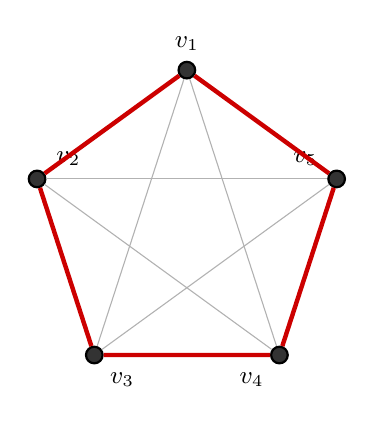
\begin{tikzpicture}[
      vertex/.style={circle, draw, fill=black!80, inner sep=0pt, minimum size=6pt},
      every node/.style={font=\small},
      thick
    ]
    % Pentagon: 5-cycle, which is Hamiltonian
    \foreach \i/\lbl in {1/$v_1$, 2/$v_2$, 3/$v_3$, 4/$v_4$, 5/$v_5$}{
      \node[vertex, label={90+72-\i*72}:{\lbl}] (v\i) at ({90+(\i-1)*72}:2cm) {};
    }
    % Hamiltonian cycle (outer pentagon) in red
    \draw[red!80!black, ultra thick]
      (v1) -- (v2) -- (v3) -- (v4) -- (v5) -- (v1);
    % Extra chords (non-Hamiltonian edges) in gray
    \draw[gray!60, thin] (v1) -- (v3);
    \draw[gray!60, thin] (v1) -- (v4);
    \draw[gray!60, thin] (v2) -- (v4);
    \draw[gray!60, thin] (v2) -- (v5);
    \draw[gray!60, thin] (v3) -- (v5);
  \end{tikzpicture}
  \caption{The Petersen-style graph (complete graph $K_5$ with Hamiltonian cycle
           highlighted). The Hamiltonian cycle $v_1 \to v_2 \to v_3 \to v_4 \to v_5
           \to v_1$ is drawn in bold red; the remaining edges of $K_5$ are shown in
           gray.}
  \label{fig:hamiltonian-cycle}
\end{figure}

\begin{figure}[htbp]
  \centering
  \begin{tikzpicture}[
      vertex/.style={circle, draw, fill=black!80, inner sep=0pt, minimum size=6pt},
      every node/.style={font=\small},
      thick
    ]
    % K_{1,4}: star graph, non-Hamiltonian (violates Dirac and Ore)
    \node[vertex, label=right:$c$] (c) at (0,0) {};
    \node[vertex, label=above:$u_1$] (u1) at (0, 2) {};
    \node[vertex, label=right:$u_2$] (u2) at (2, 0) {};
    \node[vertex, label=below:$u_3$] (u3) at (0,-2) {};
    \node[vertex, label=left:$u_4$]  (u4) at (-2,0) {};
    \draw (c) -- (u1);
    \draw (c) -- (u2);
    \draw (c) -- (u3);
    \draw (c) -- (u4);
    \node[font=\small, align=center] at (0,-3.2)
      {$\deg(c)=4$,\quad $\deg(u_i)=1$};
  \end{tikzpicture}
  \caption{The star graph $K_{1,4}$: a non-Hamiltonian graph. The central vertex $c$
           has degree $4$, while each leaf $u_i$ has degree $1 < n/2 = 5/2$, violating
           Dirac's condition. Removing $c$ disconnects the graph, so $K_{1,4}$ is not
           even $2$-connected.}
  \label{fig:non-hamiltonian}
\end{figure}

% ─── Section 3: Adjacency Matrix ──────────────────────────────────────────────
\section{Adjacency Matrix and Graph Representations}
\label{sec:adjacency}

\subsection{Definition}

\begin{definition}[Adjacency Matrix]\label{def:adj-matrix}
Let $G = (V, E)$ be a simple graph with vertex set $V = \{v_1, v_2, \ldots, v_n\}$.
The \emph{adjacency matrix} of $G$ is the $n \times n$ matrix $A = (A_{ij})$ defined by
\begin{equation}\label{eq:adj-def}
  A_{ij} =
  \begin{cases}
    1 & \text{if } \{v_i, v_j\} \in E,\\
    0 & \text{otherwise.}
  \end{cases}
\end{equation}
\end{definition}

\subsection{Properties of the Adjacency Matrix}

\begin{theorem}[Symmetry]\label{thm:adj-symmetric}
For an undirected simple graph $G$, the adjacency matrix satisfies $A = A^T$.
\end{theorem}

\begin{proof}
By Definition~\ref{def:adj-matrix}, $A_{ij} = 1$ if and only if $\{v_i, v_j\} \in E$.
Since $\{v_i, v_j\} = \{v_j, v_i\}$, we have $A_{ij} = A_{ji}$ for all $i, j$, whence
$A = A^T$.
\end{proof}

The following properties follow directly from Definition~\ref{def:adj-matrix}:

\begin{enumerate}
  \item \textbf{Zero diagonal.} For a simple graph (no loops), $A_{ii} = 0$ for all $i$.
  \item \textbf{Binary entries.} Each entry $A_{ij} \in \{0,1\}$.
  \item \textbf{Degree formula.} The degree of vertex $v_i$ is
        \begin{equation}\label{eq:degree-sum}
          \deg(v_i) = \sum_{j=1}^{n} A_{ij}.
        \end{equation}
  \item \textbf{Directed graphs.} For a directed graph (digraph), $A_{ij} = 1$ if there
        is an arc from $v_i$ to $v_j$. The matrix need not be symmetric.
\end{enumerate}

\subsection{Powers of the Adjacency Matrix}

\begin{theorem}[Walk Counting]\label{thm:adj-power}
Let $A$ be the adjacency matrix of a graph $G$. The $(i,j)$-entry of $A^k$ equals the
number of walks of length $k$ from $v_i$ to $v_j$ in $G$.
\end{theorem}

\begin{proof}
We proceed by induction on $k$.

\textbf{Base case} ($k = 1$): $(A^1)_{ij} = A_{ij}$, which equals $1$ if $\{v_i,v_j\}
\in E$ (a walk of length $1$) and $0$ otherwise. This agrees with the number of walks
of length $1$ from $v_i$ to $v_j$.

\textbf{Inductive step}: Assume the result holds for $k - 1$, i.e., $(A^{k-1})_{ij}$
counts walks of length $k-1$ from $v_i$ to $v_j$. Then
\begin{align}
  (A^k)_{ij} &= (A^{k-1} \cdot A)_{ij} \notag\\
             &= \sum_{\ell=1}^{n} (A^{k-1})_{i\ell} \cdot A_{\ell j}. \label{eq:matrix-mult}
\end{align}
A walk of length $k$ from $v_i$ to $v_j$ consists of a walk of length $k-1$ from $v_i$
to some intermediate vertex $v_\ell$, followed by a single edge $\{v_\ell, v_j\}$.
By the inductive hypothesis, $(A^{k-1})_{i\ell}$ counts such walks of length $k-1$,
and $A_{\ell j}$ equals $1$ if $\{v_\ell, v_j\} \in E$ (and $0$ otherwise). Summing
over all possible intermediate vertices $v_\ell$ yields the total number of walks of
length $k$ from $v_i$ to $v_j$, which equals $(A^k)_{ij}$.
\end{proof}

\subsection{Adjacency List vs.\ Adjacency Matrix}

\begin{remark}[Space Complexity Comparison]\label{rem:adj-list-vs-matrix}
Two common graph representations are:
\begin{itemize}
  \item \textbf{Adjacency matrix.} Requires $\Theta(n^2)$ space. Entry lookup is $O(1)$.
        Efficient for dense graphs ($|E| = \Theta(n^2)$) or when frequent edge queries
        are required.
  \item \textbf{Adjacency list.} Requires $\Theta(n + m)$ space, where $m = |E|$.
        Traversal of all neighbours of a vertex is $O(\deg(v))$. Efficient for sparse
        graphs.
\end{itemize}
For most algorithmic applications in sparse graphs (e.g., shortest paths, graph
traversal), the adjacency list representation is preferred.
\end{remark}

\subsection{Worked Examples}

\subsubsection{Undirected Graph}

\begin{figure}[htbp]
  \centering
  \begin{minipage}{0.45\textwidth}
    \centering
    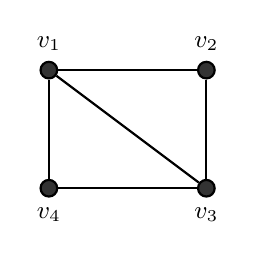
\begin{tikzpicture}[
        vertex/.style={circle, draw, fill=black!80, inner sep=0pt, minimum size=6pt},
        every node/.style={font=\small},
        thick
      ]
      \node[vertex, label=above:$v_1$] (v1) at (0,1.5) {};
      \node[vertex, label=above:$v_2$] (v2) at (2,1.5) {};
      \node[vertex, label=below:$v_3$] (v3) at (2,0)   {};
      \node[vertex, label=below:$v_4$] (v4) at (0,0)   {};
      \draw (v1) -- (v2);
      \draw (v2) -- (v3);
      \draw (v3) -- (v4);
      \draw (v4) -- (v1);
      \draw (v1) -- (v3);
    \end{tikzpicture}
    \par\vspace{4pt}
    {\small Undirected graph $G$}
  \end{minipage}
  \hfill
  \begin{minipage}{0.45\textwidth}
    \centering
    \[
      A =
      \begin{pmatrix}
        0 & 1 & 1 & 1 \\
        1 & 0 & 1 & 0 \\
        1 & 1 & 0 & 1 \\
        1 & 0 & 1 & 0
      \end{pmatrix}
    \]
    \par\vspace{4pt}
    {\small Adjacency matrix of $G$}
  \end{minipage}
  \caption{An undirected graph $G$ on four vertices (left) and its adjacency matrix $A$
           (right). Observe that $A = A^T$ (Theorem~\ref{thm:adj-symmetric}), and
           $\deg(v_1) = \sum_j A_{1j} = 3$ (row sum). The entry $(A^2)_{13}$ counts
           the number of walks of length $2$ from $v_1$ to $v_3$.}
  \label{fig:adj-matrix-undirected}
\end{figure}

\subsubsection{Directed Graph}

\begin{figure}[htbp]
  \centering
  \begin{minipage}{0.45\textwidth}
    \centering
    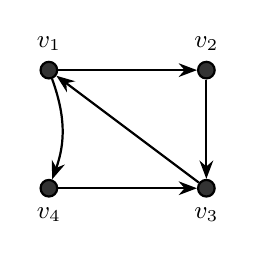
\begin{tikzpicture}[
        vertex/.style={circle, draw, fill=black!80, inner sep=0pt, minimum size=6pt},
        every node/.style={font=\small},
        ->, >=Stealth, thick
      ]
      \node[vertex, label=above:$v_1$] (v1) at (0,1.5) {};
      \node[vertex, label=above:$v_2$] (v2) at (2,1.5) {};
      \node[vertex, label=below:$v_3$] (v3) at (2,0)   {};
      \node[vertex, label=below:$v_4$] (v4) at (0,0)   {};
      \draw (v1) -- (v2);
      \draw (v2) -- (v3);
      \draw (v3) -- (v1);
      \draw (v4) -- (v3);
      \draw (v1) to[bend left=20] (v4);
    \end{tikzpicture}
    \par\vspace{4pt}
    {\small Directed graph $D$}
  \end{minipage}
  \hfill
  \begin{minipage}{0.45\textwidth}
    \centering
    \[
      A_D =
      \begin{pmatrix}
        0 & 1 & 0 & 1 \\
        0 & 0 & 1 & 0 \\
        1 & 0 & 0 & 0 \\
        0 & 0 & 1 & 0
      \end{pmatrix}
    \]
    \par\vspace{4pt}
    {\small Adjacency matrix of $D$}
  \end{minipage}
  \caption{A directed graph $D$ on four vertices (left) and its adjacency matrix $A_D$
           (right). Note that $A_D \neq A_D^T$, reflecting the asymmetry of directed
           edges. For instance, there is an arc from $v_1$ to $v_4$ but no arc from
           $v_4$ to $v_1$, giving $(A_D)_{14} = 1$ and $(A_D)_{41} = 0$.}
  \label{fig:adj-matrix-directed}
\end{figure}

\begin{example}[Computing $A^2$]\label{ex:A-squared}
For the undirected graph $G$ in Figure~\ref{fig:adj-matrix-undirected}, one computes
\begin{equation}
  A^2 =
  \begin{pmatrix}
    3 & 1 & 2 & 1 \\
    1 & 2 & 1 & 2 \\
    2 & 1 & 3 & 1 \\
    1 & 2 & 1 & 2
  \end{pmatrix}.
\end{equation}
The entry $(A^2)_{13} = 2$ indicates that there are exactly $2$ walks of length $2$
from $v_1$ to $v_3$: namely $v_1 \to v_2 \to v_3$ and $v_1 \to v_4 \to v_3$.
By Theorem~\ref{thm:adj-power}, this count is exact.
\end{example}

\end{document}